% !TeX root = ../Tempel-Daniel.tex
\chapter{RAG and Agentic Retrieval}
\label{chap:retrieval}

The previous chapter established that the active context of the AI Software Engineering Assistant should contain information relevant to the model’s current decision rather than all information available to the runtime. A software repository creates the corresponding retrieval problem: a task may depend on only a few methods, tests or configuration files, while the complete repository may contain thousands of files. The challenge is therefore not simply to provide the LLM with more context, but to locate the external evidence relevant to the current task.

\textcite{lewis2020rag} introduced Retrieval-Augmented Generation (RAG) by combining parametric model knowledge with information retrieved from an external non-parametric source. The original work used a neural retriever and dense index. This chapter uses RAG in the broader architectural sense common in current LLM systems: generation is augmented with externally retrieved information at inference time. For a software-engineering assistant, such sources can include repository files, documentation and project knowledge that change independently from model parameters.

\section{Repository-aware retrieval}
\label{sec:repository-retrieval}

Retrieval does not necessarily require a separately constructed vector index. Direct text or symbol search can operate on current repository files, while indexed systems prepare searchable representations in advance. The appropriate approach depends on repository size, task requirements and measured retrieval quality.

Indexed retrieval typically divides source material into searchable units and associates them with metadata such as file path, module, class or symbol. Source code makes this more difficult than prose because useful information follows program structure rather than arbitrary token boundaries. Structure-aware chunking can preserve boundaries such as functions or methods, but retrieval units must remain small enough to search efficiently while retaining enough surrounding information to be interpretable.

Repository search can use several relevance signals. Lexical retrieval is effective for exact identifiers, exception names, configuration keys or error messages. BM25 is a widely used lexical ranking method and remains a strong baseline across heterogeneous retrieval tasks \parencite{thakur2021beir}.

Lexical overlap becomes less reliable when the task and implementation use different terminology. A user may describe authentication behaviour while the repository represents it through identifiers such as \texttt{validateBearerToken} or \texttt{securityContext}. Dense retrieval addresses this mismatch by representing queries and searchable units as embeddings. CodeSearchNet illustrates this problem directly: semantic code search must connect natural-language descriptions with the technical vocabulary used in source code \parencite{husain2019codesearchnet}.

Repository structure can provide another useful signal. Source files are connected through calls, imports, symbol references, inheritance and test–implementation relationships. If retrieval identifies a function in \texttt{src/auth.py}, its callers, validation helpers or related tests may be more useful than unrelated code with similar wording. RepoGraph explores this principle by representing repository-level relationships as a graph for AI software-engineering tasks \parencite{ouyang2025repograph}. Such structural information requires additional analysis and may be incomplete.

Lexical, dense and structural retrieval should therefore be treated as complementary options rather than mandatory stages. A retrieval subsystem can select or combine them according to the repository, task and evaluation results. An indexed system may also retrieve a broad candidate set and then apply a reranker to a smaller subset. A reranker may improve ranking quality at additional computational cost \parencite{thakur2021beir}.

Figure~\ref{fig:rag-agentic-retrieval} shows direct and indexed routes to repository evidence; the feedback path allows further retrieval when the current evidence is insufficient.

\begin{figure}[!htbp]
\centering
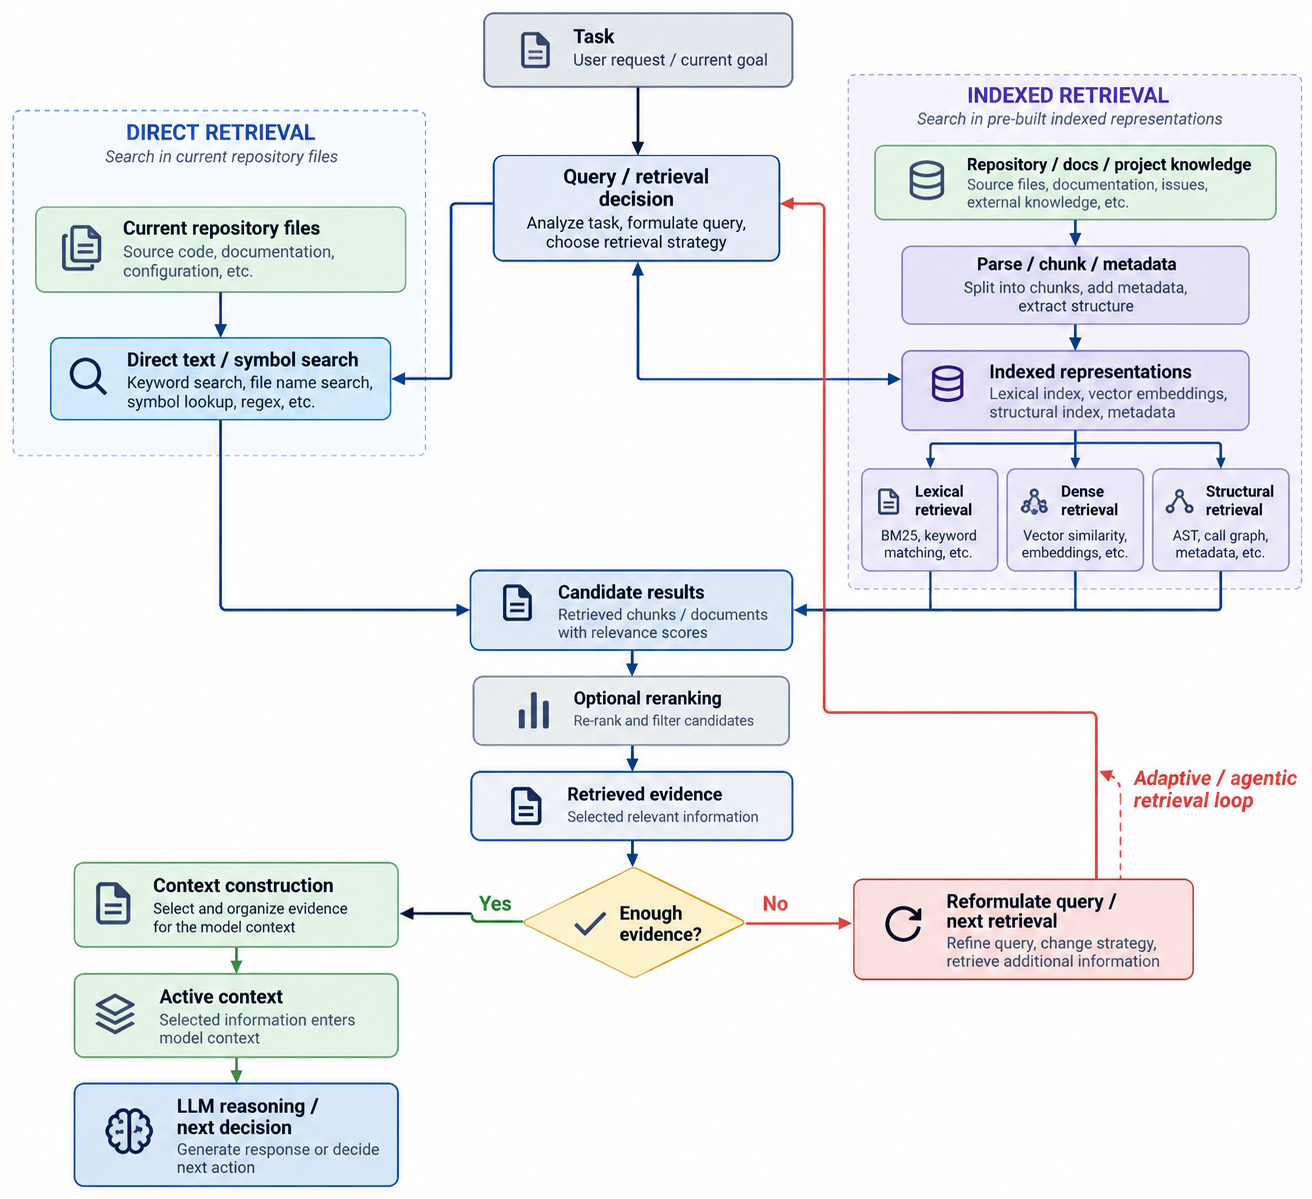
\includegraphics[width=\linewidth]{images/rag-agentic-retrieval.png}
\caption{Direct and indexed repository retrieval for the AI Software Engineering Assistant, including optional lexical, dense and structural search, reranking and adaptive additional retrieval.}
\label{fig:rag-agentic-retrieval}
\end{figure}

\noindent\begin{minipage}{\linewidth}
Table~\ref{tab:retrieval-signals} summarises the uses and limitations of these complementary retrieval signals.\par\vspace{5pt}
\captionsetup{hypcap=false}
\captionof{table}{Retrieval signals for repository tasks and their typical limitations.}
\label{tab:retrieval-signals}
\small\singlespacing
\renewcommand{\arraystretch}{1.15}
\begin{tabular}{@{}p{2.7cm}p{6.0cm}p{6.8cm}@{}}
\toprule
{\raggedright\textbf{Retrieval signal}\par} & {\raggedright\textbf{Useful for repository tasks}\par} & {\raggedright\textbf{Typical limitation}\par} \\
\midrule
{\raggedright Lexical retrieval\par} & {\raggedright Exact symbols, identifiers and error messages\par} & {\raggedright Limited when query and implementation use different terminology\par} \\
{\raggedright Dense retrieval\par} & {\raggedright Semantic similarity between natural language and source code\par} & {\raggedright May rank semantically related but incorrect identifiers highly\par} \\
{\raggedright Structural retrieval\par} & {\raggedright Calls, imports, references and test–implementation relationships\par} & {\raggedright Requires additional analysis and may be incomplete\par} \\
\bottomrule
\end{tabular}
\end{minipage}

Retrieved results should be treated as external evidence rather than as the complete model context. For the recurring task \emph{Fix GitHub issue \#42 and verify the solution}, an initial search for \texttt{Authorization} may locate \texttt{src/auth.py} and related tests. These results can then be passed to the context-building stage described in Chapter~\ref{chap:context-memory} together with the issue description and current task state.

\section{From iterative retrieval to agentic retrieval}
\label{sec:agentic-retrieval}

{\setlength{\emergencystretch}{2em}
A single retrieval operation is sufficient when the information need is already clear. Repository-level tasks are often less direct because an issue describes observed behaviour while relevant implementation details become visible only after part of the repository has been inspected.\par}

Suppose issue \#42 reports that an \texttt{Authorization} header is handled incorrectly. The assistant may first search for \texttt{Authorization} and inspect \texttt{src/auth.py}. That file may reveal a separate token-validation function, whose implementation and references lead to middleware configuration or tests defining the expected behaviour. The useful search sequence therefore cannot always be formulated completely from the original issue description.

This creates an iterative process:

\begin{center}
\small\singlespacing
search \(\rightarrow\) inspect evidence \(\rightarrow\) identify missing information
\\ \(\rightarrow\) reformulate the search \(\rightarrow\) retrieve again.
\end{center}

RepoCoder applies a related principle to repository-level code completion by alternating retrieval and generation. Its experiments showed improvements over the vanilla retrieval-augmented baseline evaluated in that work \parencite{zhang2023repocoder}. This supports iterative use of newly discovered information, but does not by itself demonstrate the benefit of autonomous retrieval decisions for issue-resolution tasks.

Iteration alone does not make retrieval agentic. A fixed pipeline could always perform several searches without making adaptive decisions. Here, \textbf{agentic retrieval} refers to retrieval in which subsequent search decisions depend on intermediate evidence. The model or surrounding runtime can decide whether another search is required, what information is missing, which retrieval mechanism to use and when sufficient evidence has been collected.

Recent work on Agentic RAG describes a broader transition from fixed pipelines toward systems that adapt retrieval strategies and refine queries across multiple evidence-gathering steps \parencite{singh2025agenticrag}. Agentic retrieval refers here to the retrieval component of this behaviour, while Agentic RAG describes the wider interaction between adaptive retrieval, generation and reasoning.

Adaptive steps may combine direct text or symbol search with indexed lexical, dense or structural retrieval. Editing, testing and task completion belong to the broader agent loop described in Chapter~\ref{chap:agents}.

Adaptive retrieval adds cost and failure modes. Query reformulation can drift away from the original task, repeated searches can return the same evidence and unnecessary retrieval rounds increase latency and model usage. A failed search also does not establish that no relevant implementation exists; another query or retrieval method may still locate it. Retrieval budgets and tracking of previously inspected results can therefore limit unnecessary search.

\section{Retrieval reliability}
\label{sec:retrieval-reliability}

Retrieval quality depends not only on relevance but also on whether the retrieved information corresponds to the repository state on which the assistant operates. An index is a derived representation of repository content and can become stale when files change.

Repository, branch and commit metadata can identify the source snapshot from which indexed information was produced. A commit, however, does not represent uncommitted working-tree changes. Because operations such as \texttt{apply\_patch} modify files before a new commit necessarily exists, relevant indexed results should be checked against the current working-tree files before they are used to justify an edit.

Incremental indexing can update affected entries and relationships after files are added, modified or deleted rather than rebuilding the complete index after every change. Structural indexes require particular care because a change in one file can alter relationships to symbols elsewhere.

Not every form of current state belongs in a retrieval index. Frequently changing operational information such as Git status, test output or CI results can be obtained directly through tools. Retrieval is more appropriate for searching larger collections of source code, documentation and project knowledge.

Retrieval should also be evaluated separately from the LLM that consumes its results. A failure caused by missing evidence differs from one in which correct evidence was retrieved but interpreted incorrectly. Retrieval can also succeed while the context-building stage excludes the relevant result. Component-level evaluation therefore helps distinguish these failure sources by recording both retrieved evidence and the information actually included in the active context.

For a single ranked retrieval operation, Recall@k measures the proportion of annotated relevant retrieval units found among the top-k results. The retrieval unit may be a file, method or chunk and must be defined together with the relevance labels used by the evaluation set. A ranking metric such as nDCG@k can additionally account for graded relevance and result position.

An agentic retrieval strategy may execute several queries and combine evidence across multiple steps. It should therefore also be evaluated at task level under a defined retrieval or tool budget. Relevant measures include whether the required evidence was eventually acquired, retrieval latency, the number of retrieval rounds and, ultimately, whether the complete assistant succeeds on realistic software-engineering tasks.

Repository characteristics and evaluation results should determine which retrieval mechanisms and degree of adaptation are useful. The following chapter examines the Model Context Protocol as a standardised interface for exposing repository resources and retrieval tools to the assistant runtime.
